\subsubsection{Giới thiệu}
Mô hình Sequence-to-Sequence (Seq2Seq) nhận input là một sequence và trả lại output cũng là một sequence. Ví dụ bài toán QA, input là câu hỏi "how are you?" và output là câu trả lời "I am good". Phương pháp truyền thống sử dụng RNNs cho cả encoder (phần mã hóa input) và decoder (phần giải mã input và đưa ra output tương ứng).

Nhưng mô hình này vẫn có nhiều điểm yếu như đã trình bày, điểm yếu thứ nhất của RNNs là thời gian train rất chậm, đến mức người ta phải sử dụng phiên bản Truncated Backpropagation để train nó. Mặc dù vậy, tốc độ train vẫn rất chậm do phải sử dụng CPU, không tận dụng được tính toán song song trên GPU.  Điểm yếu thứ hai là nó xử lý không tốt với những câu dài do hiện tượng Gradient Vanishing/Exploding. Khi số lượng units càng lớn, gradient giảm dần ở các units cuối do công thức Đạo hàm chuỗi, dẫn đến mất thông tin/sự phụ thuộc xa giữa các units.

Ra đời năm 1991, Long-short Term Memory (LSTM) có vẻ đã giải quyết phần nào vẫn đề Gradient Vanishing, nhưng LSTM lại phức tạp hơn RNNs rất nhiều, và hiển nhiên nó cũng train chậm hơn RNN đáng kể.

Vậy có cách nào tận dụng khả năng tính toán song song của GPU để tăng tốc độ train cho các mô hình ngôn ngữ, đồng thời khắc phục điểm yếu xử lý câu dài không? Transformers chính là câu trả lời. Ý tưởng chính của phần này được lấy từ bài báo Attention is all you need[xxx] giới thiệu về các cơ chế attention  được sử dụng trong các tác vụ học máy.

Điều đặc biệt về Transformer so với mô hình RNN là nó không yêu cầu xử lý các phần tử trong chuỗi một cách tuần tự. Trong khi RNN phải xử lý từng phần tử theo thứ tự từ đầu đến cuối, Transformer có thể xử lý toàn bộ câu ngôn ngữ tự nhiên cùng một lúc. Điều này cho phép Transformer tận dụng tối đa khả năng tính toán song song của GPU và giảm thời gian xử lý đáng kể. Thay vì phải chờ đợi kết quả từ các phần tử trước đó trong chuỗi, Transformer có thể đồng thời xem xét và ánh xạ mối quan hệ giữa tất cả các từ trong câu. Điều này giúp mô hình hiểu được mối quan hệ toàn diện trong câu và tạo ra các biểu diễn ngữ nghĩa phong phú hơn.

Transformer hoạt động dựa trên cơ chế attention, trong đó mỗi từ trong câu được so sánh với tất cả các từ khác để xác định mức độ quan trọng của từ đó đối với các từ khác. Quá trình attention này cho phép mô hình tập trung vào các từ quan trọng và xây dựng biểu diễn phản ánh mối quan hệ giữa chúng. Đồng thời, Transformer sử dụng các lớp mạng nơ-ron đầy đủ để thực hiện biến đổi phi tuyến trên biểu diễn từ sau quá trình attention.

\subsubsection{Kiến trúc Tranformer}
\begin{figure}[htb]
    \centering
    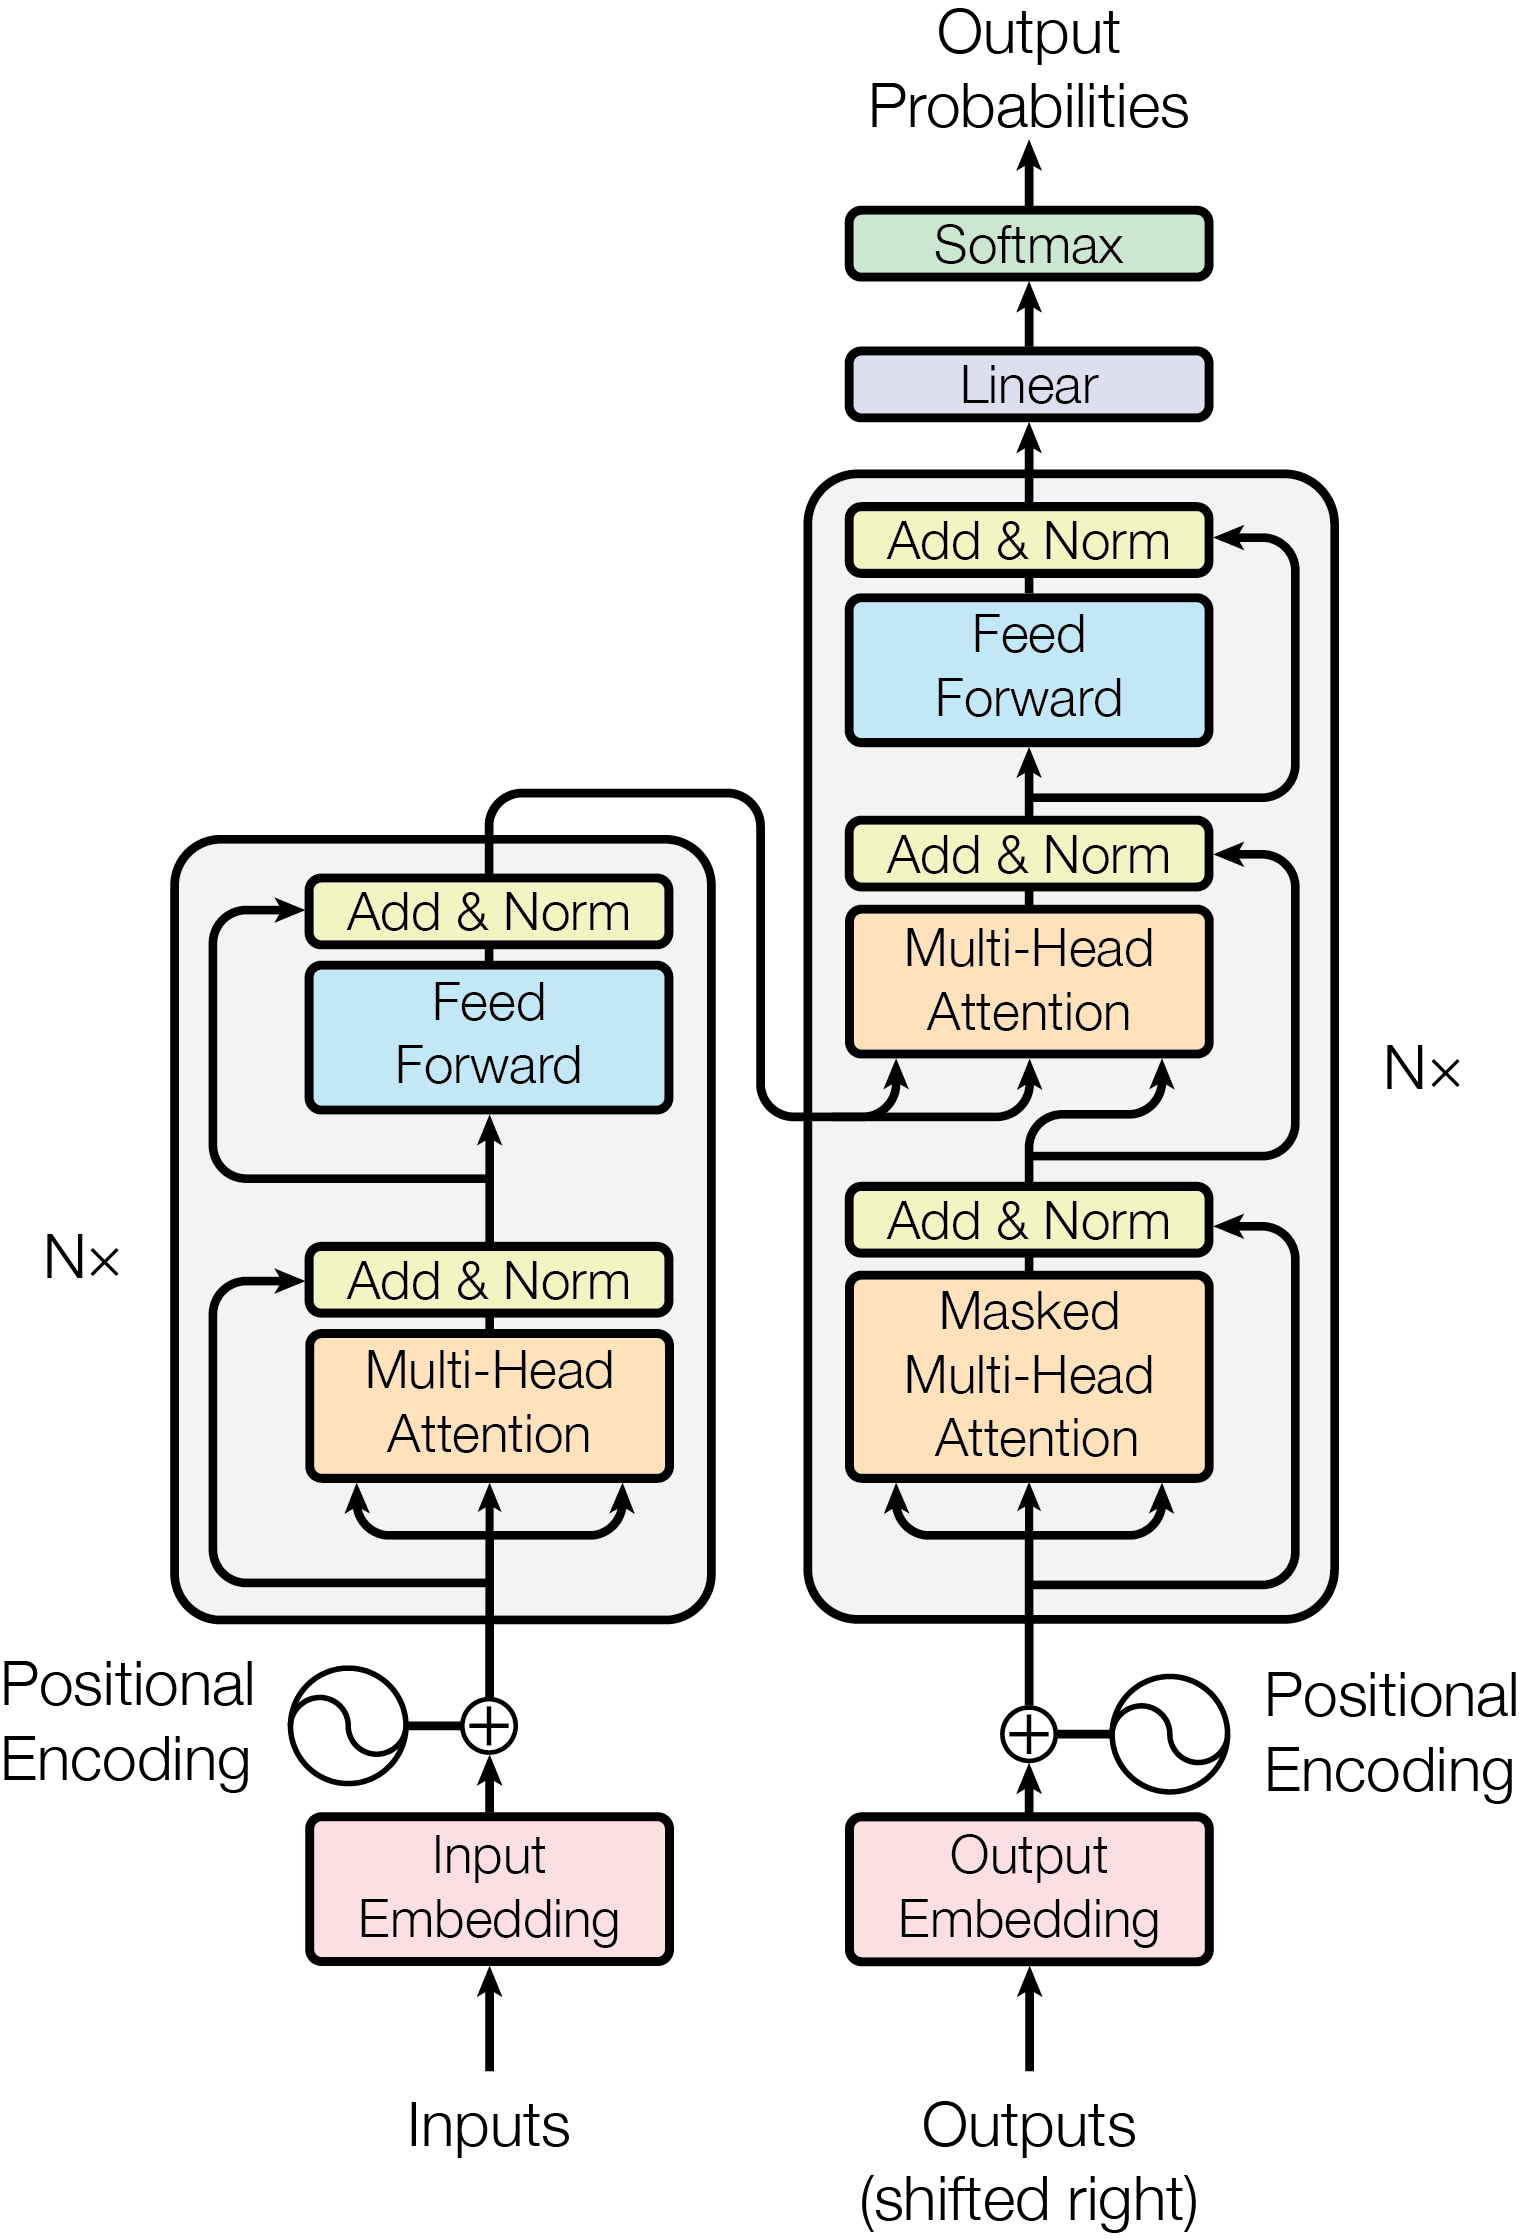
\includegraphics[width=\textwidth]{image/tranformer-architecture.png}
    \caption{Kiến trúc của mô hình Tranformer}
    \label{figure:tranformer-architecture}
\end{figure}



Kiến trúc này gồm 2 phần encoder bên trái và decoder bên phải.

\textbf{Encoder}: là tổng hợp xếp chồng lên nhau của 6 layers xác định. Mỗi layer bao gồm 2 layer con (sub-layer) trong nó. Sub-layer đầu tiên là multi-head self-attention mà lát nữa chúng ta sẽ tìm hiểu. Layer thứ 2 đơn thuần chỉ là các fully-connected feed-forward layer. Một lưu ý là chúng ta sẽ sử dụng một kết nối residual ở mỗi sub-layer ngay sau layer normalization. Kiến trúc này có ý tưởng tương tự như mạng resnet trong CNN. Đầu ra của mỗi sub-layer là $LayerNorm(x+Sublayer(x))$ có số chiều là 512 theo như bài viết.

\textbf{Decoder}: Decoder cũng là tổng hợp xếp chồng của 6 layers. Kiến trúc tương tự như các sub-layer ở Encoder ngoại trừ thêm 1 sub-layer thể hiện phân phối attention ở vị trí đầu tiên. Layer này không gì khác so với multi-head self-attention layer ngoại trừ được điều chỉnh để không đưa các từ trong tương lai vào attention. Tại bước thứ $i$ của decoder chúng ta chỉ biết được các từ ở vị trí nhỏ hơn $i$ nên việc điều chỉnh đảm bảo attention chỉ áp dụng cho những từ nhỏ hơn vị trí thứ $i$. Cơ chế residual cũng được áp dụng tương tự như trong Encoder.

Ngoài ra luôn có một bước cộng thêm Positional Encoding vào các input của encoder và decoder nhằm đưa thêm yếu tố thời gian vào mô hình làm tăng độ chuẩn xác. Đây chỉ đơn thuần là phép cộng vector mã hóa vị trí của từ trong câu với vector biểu diễn từ. Chúng ta có thể mã hóa dưới dạng $[0, 1]$ vector vị trí hoặc sử dụng hàm $sin,cos$ như trong bài báo.

\subsubsection{Cơ chế Attention}
\begin{enumerate}
    \item {Scaled Dot-Product Attention}

    Đây chính là một cơ chế self-attention khi mỗi từ có thể điều chỉnh trọng số của nó cho các từ khác trong câu sao cho từ ở vị trí càng gần nó nhất thì trọng số càng lớn và càng xa thì càng nhỏ dần. Sau bước nhúng từ (đi qua embeding layer) ta có đầu vào của encoder và decoder là ma trận $\mathbf{X}$ kích thước $m\times n$, $m,n$ lần lượt là là độ dài câu và số chiều của một vector nhúng từ.

    Sau đó, ma trận $\mathbf{X}$ sẽ được nhân với 3 ma trận trọng số tương ứng $\mathbf{W}_\mathbf{q}$, $\mathbf{W}_\mathbf{k}$, $\mathbf{W}_\mathbf{v}$ chính là những hệ số mà model cần huấn luyện, ta thu được ma trận $\mathbf{Q}$, $\mathbf{K}$, $\mathbf{V}$ (Query, Key và Value). Ma trận Query và Key có tác dụng tính toán ra phân phối score cho các cặp từ. Ma trận Value sẽ dựa trên phân phối score để tính ra véc tơ phân phối xác suất output. Ba ma trận $\mathbf{Q}$, $\mathbf{K}$, $\mathbf{V}$ chính là 3 mũi tên đầu vào của các Multi-head Attention (bản chất là Self-Attention) trong kiến trúc tổng quát hình x.

    Như đã đề cập, Đầu vào để tính attention sẽ bao gồm ma trận $\mathbf{Q}$ (mỗi dòng của nó là một vector query đại diện cho các từ input), ma trận $\mathbf{K}$ (tương tự như ma trận $\mathbf{Q}$, mỗi dòng là vector key đại diện cho các từ input). Hai ma trận $\mathbf{Q}$, $\mathbf{K}$ được sử dụng để tính attention mà các từ trong câu trả về cho 1 từ cụ thể trong câu. Attention vector sẽ được tính dựa trên trung bình có trọng số của các vector value trong ma trận $\mathbf{V}$ với trọng số attention (được tính từ $\mathbf{Q}$, $\mathbf{K}$).

    Phương trình Attention như sau:
    \begin{align}
        \mathrm{Attention}({Q, K, V}) = \mathrm{softmax}(\frac{{QK^T})}{\sqrt{d_k}}\ {V} \tag{xxx}
    \end{align}

    Việc chia cho $d_k$ là số dimension của vector key nhằm mục đích tránh tràn luồng nếu số mũ là quá lớn.
    Trong thực hành chúng ta tính toán hàm attention trên toàn bộ tập các câu truy vấn một cách đồng thời được đóng gói thông qua ma trận $\mathbf{Q}$. Keys và Values cũng được đóng gói cùng nhau thông qua ma trận $\mathbf{K},\mathbf{V}$.

    \begin{figure}[htb]
        \centering
        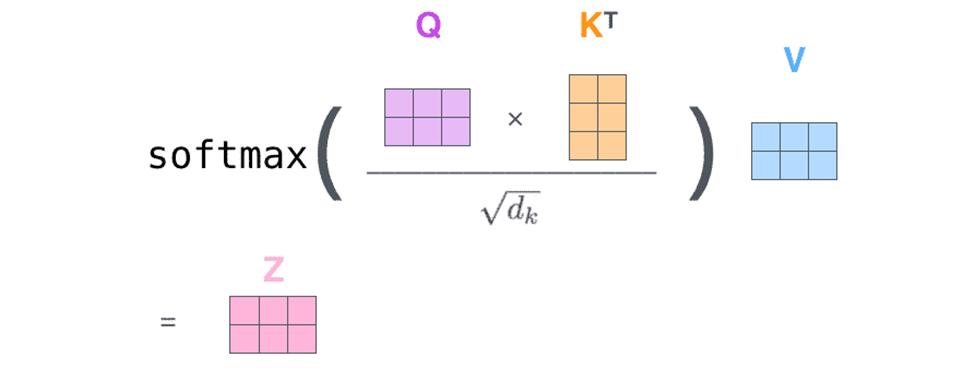
\includegraphics[width=\textwidth]{image/attention-equation.png}
        \caption{Phương trình Attention thể hiện dưới dạng ma trận}
        \label{figure:attention-equation}
    \end{figure}

    \item {Multi-head Attention}
    
    Như vậy sau quá trình Scale dot production chúng ta sẽ thu được 1 ma trận attention. Các tham số mà model cần tinh chỉnh chính là các ma trận $\mathbf{W}_\mathbf{q},\mathbf{W}_\mathbf{k},\mathbf{W}_\mathbf{v}$. Mỗi quá trình như vậy được gọi là một head của attention. Khi lặp lại quá trình này nhiều lần (trong bài báo là ba heads) ta sẽ thu được quá trình Multi-head Attention.
    
    Sau khi thu được ba ma trận attention ở đầu ra chúng ta sẽ concatenate các matrix này theo các cột để thu được ma trận tổng hợp multi-head matrix có chiều cao trùng với chiều cao của ma trận input.
    
    \begin{align*}
        \mathrm{MultiHead}(Q, K, V) &= \mathrm{Concat}({head_1},{head_2}, ..., {head_h})W^O\\
    %    \mathrm{where} \mathrm{head_i} &= \mathrm{Attention}(QW_Q_i^{\dmodel \times d_q}, KW_K_i^{\dmodel \times d_k}, VW^V_i^{\dmodel \times d_v})\\
        \text{với}~{head_i} &= \mathrm{Attention}(QW^Q_i, KW^K_i, VW^V_i)\\
    \end{align*}
    

    Cuối cùng, để trả về output có cùng kích thước với ma trận input chúng ta chỉ cần nhân với ma trận $\mathbf{W}_\mathbf{0}$ có chiều rộng bằng với chiều rộng của ma trận input.

    \begin{figure}[htb]
        \centering
        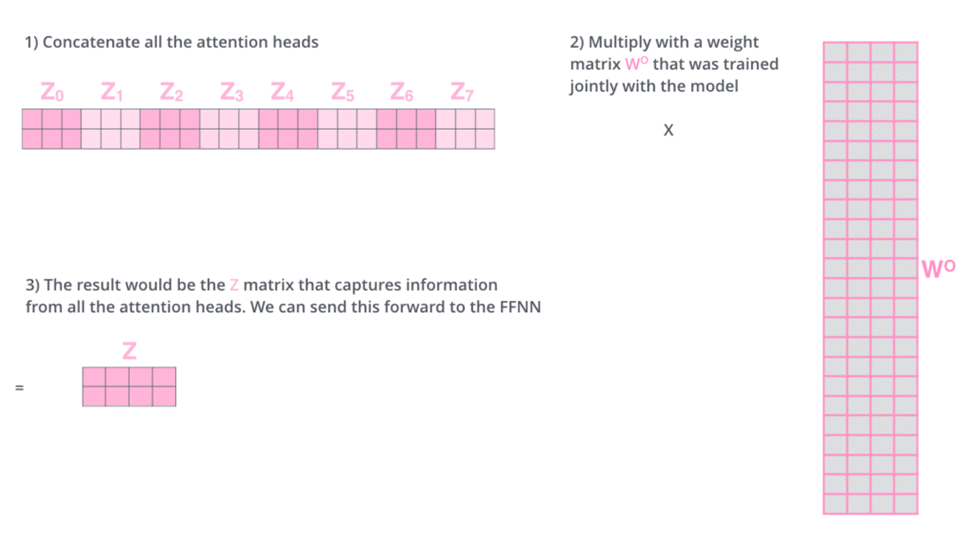
\includegraphics[width=\textwidth]{image/multi-head-illustration.png}
        \caption{Multi-head Attention minh hoạ dưới dạng ma trận}
        \label{figure:multi-head-illustration}
    \end{figure}

\end{enumerate}
